% Options for packages loaded elsewhere
\PassOptionsToPackage{unicode}{hyperref}
\PassOptionsToPackage{hyphens}{url}
%
\documentclass[
]{book}
\usepackage{amsmath,amssymb}
\usepackage{iftex}
\ifPDFTeX
  \usepackage[T1]{fontenc}
  \usepackage[utf8]{inputenc}
  \usepackage{textcomp} % provide euro and other symbols
\else % if luatex or xetex
  \usepackage{unicode-math} % this also loads fontspec
  \defaultfontfeatures{Scale=MatchLowercase}
  \defaultfontfeatures[\rmfamily]{Ligatures=TeX,Scale=1}
\fi
\usepackage{lmodern}
\ifPDFTeX\else
  % xetex/luatex font selection
\fi
% Use upquote if available, for straight quotes in verbatim environments
\IfFileExists{upquote.sty}{\usepackage{upquote}}{}
\IfFileExists{microtype.sty}{% use microtype if available
  \usepackage[]{microtype}
  \UseMicrotypeSet[protrusion]{basicmath} % disable protrusion for tt fonts
}{}
\makeatletter
\@ifundefined{KOMAClassName}{% if non-KOMA class
  \IfFileExists{parskip.sty}{%
    \usepackage{parskip}
  }{% else
    \setlength{\parindent}{0pt}
    \setlength{\parskip}{6pt plus 2pt minus 1pt}}
}{% if KOMA class
  \KOMAoptions{parskip=half}}
\makeatother
\usepackage{xcolor}
\usepackage{color}
\usepackage{fancyvrb}
\newcommand{\VerbBar}{|}
\newcommand{\VERB}{\Verb[commandchars=\\\{\}]}
\DefineVerbatimEnvironment{Highlighting}{Verbatim}{commandchars=\\\{\}}
% Add ',fontsize=\small' for more characters per line
\usepackage{framed}
\definecolor{shadecolor}{RGB}{248,248,248}
\newenvironment{Shaded}{\begin{snugshade}}{\end{snugshade}}
\newcommand{\AlertTok}[1]{\textcolor[rgb]{0.94,0.16,0.16}{#1}}
\newcommand{\AnnotationTok}[1]{\textcolor[rgb]{0.56,0.35,0.01}{\textbf{\textit{#1}}}}
\newcommand{\AttributeTok}[1]{\textcolor[rgb]{0.13,0.29,0.53}{#1}}
\newcommand{\BaseNTok}[1]{\textcolor[rgb]{0.00,0.00,0.81}{#1}}
\newcommand{\BuiltInTok}[1]{#1}
\newcommand{\CharTok}[1]{\textcolor[rgb]{0.31,0.60,0.02}{#1}}
\newcommand{\CommentTok}[1]{\textcolor[rgb]{0.56,0.35,0.01}{\textit{#1}}}
\newcommand{\CommentVarTok}[1]{\textcolor[rgb]{0.56,0.35,0.01}{\textbf{\textit{#1}}}}
\newcommand{\ConstantTok}[1]{\textcolor[rgb]{0.56,0.35,0.01}{#1}}
\newcommand{\ControlFlowTok}[1]{\textcolor[rgb]{0.13,0.29,0.53}{\textbf{#1}}}
\newcommand{\DataTypeTok}[1]{\textcolor[rgb]{0.13,0.29,0.53}{#1}}
\newcommand{\DecValTok}[1]{\textcolor[rgb]{0.00,0.00,0.81}{#1}}
\newcommand{\DocumentationTok}[1]{\textcolor[rgb]{0.56,0.35,0.01}{\textbf{\textit{#1}}}}
\newcommand{\ErrorTok}[1]{\textcolor[rgb]{0.64,0.00,0.00}{\textbf{#1}}}
\newcommand{\ExtensionTok}[1]{#1}
\newcommand{\FloatTok}[1]{\textcolor[rgb]{0.00,0.00,0.81}{#1}}
\newcommand{\FunctionTok}[1]{\textcolor[rgb]{0.13,0.29,0.53}{\textbf{#1}}}
\newcommand{\ImportTok}[1]{#1}
\newcommand{\InformationTok}[1]{\textcolor[rgb]{0.56,0.35,0.01}{\textbf{\textit{#1}}}}
\newcommand{\KeywordTok}[1]{\textcolor[rgb]{0.13,0.29,0.53}{\textbf{#1}}}
\newcommand{\NormalTok}[1]{#1}
\newcommand{\OperatorTok}[1]{\textcolor[rgb]{0.81,0.36,0.00}{\textbf{#1}}}
\newcommand{\OtherTok}[1]{\textcolor[rgb]{0.56,0.35,0.01}{#1}}
\newcommand{\PreprocessorTok}[1]{\textcolor[rgb]{0.56,0.35,0.01}{\textit{#1}}}
\newcommand{\RegionMarkerTok}[1]{#1}
\newcommand{\SpecialCharTok}[1]{\textcolor[rgb]{0.81,0.36,0.00}{\textbf{#1}}}
\newcommand{\SpecialStringTok}[1]{\textcolor[rgb]{0.31,0.60,0.02}{#1}}
\newcommand{\StringTok}[1]{\textcolor[rgb]{0.31,0.60,0.02}{#1}}
\newcommand{\VariableTok}[1]{\textcolor[rgb]{0.00,0.00,0.00}{#1}}
\newcommand{\VerbatimStringTok}[1]{\textcolor[rgb]{0.31,0.60,0.02}{#1}}
\newcommand{\WarningTok}[1]{\textcolor[rgb]{0.56,0.35,0.01}{\textbf{\textit{#1}}}}
\usepackage{longtable,booktabs,array}
\usepackage{calc} % for calculating minipage widths
% Correct order of tables after \paragraph or \subparagraph
\usepackage{etoolbox}
\makeatletter
\patchcmd\longtable{\par}{\if@noskipsec\mbox{}\fi\par}{}{}
\makeatother
% Allow footnotes in longtable head/foot
\IfFileExists{footnotehyper.sty}{\usepackage{footnotehyper}}{\usepackage{footnote}}
\makesavenoteenv{longtable}
\usepackage{graphicx}
\makeatletter
\newsavebox\pandoc@box
\newcommand*\pandocbounded[1]{% scales image to fit in text height/width
  \sbox\pandoc@box{#1}%
  \Gscale@div\@tempa{\textheight}{\dimexpr\ht\pandoc@box+\dp\pandoc@box\relax}%
  \Gscale@div\@tempb{\linewidth}{\wd\pandoc@box}%
  \ifdim\@tempb\p@<\@tempa\p@\let\@tempa\@tempb\fi% select the smaller of both
  \ifdim\@tempa\p@<\p@\scalebox{\@tempa}{\usebox\pandoc@box}%
  \else\usebox{\pandoc@box}%
  \fi%
}
% Set default figure placement to htbp
\def\fps@figure{htbp}
\makeatother
\setlength{\emergencystretch}{3em} % prevent overfull lines
\providecommand{\tightlist}{%
  \setlength{\itemsep}{0pt}\setlength{\parskip}{0pt}}
\setcounter{secnumdepth}{5}
\usepackage{booktabs}
\usepackage{amsthm}
\makeatletter
\def\thm@space@setup{%
  \thm@preskip=8pt plus 2pt minus 4pt
  \thm@postskip=\thm@preskip
}
\makeatother
\usepackage[]{natbib}
\bibliographystyle{apalike}
\usepackage{bookmark}
\IfFileExists{xurl.sty}{\usepackage{xurl}}{} % add URL line breaks if available
\urlstyle{same}
\hypersetup{
  pdftitle={Ánalisis exploratorio con variable respuesta numérica: prueba con el conjunto de datos 'California Housing},
  pdfauthor={Karina Núñez Sarmiento, Isabella Sandoval Escorcia},
  hidelinks,
  pdfcreator={LaTeX via pandoc}}

\title{Ánalisis exploratorio con variable respuesta numérica: prueba con el conjunto de datos 'California Housing}
\author{Karina Núñez Sarmiento, Isabella Sandoval Escorcia}
\date{2026-08-08}

\begin{document}
\maketitle

{
\setcounter{tocdepth}{1}
\tableofcontents
}
\begin{Shaded}
\begin{Highlighting}[]
\FunctionTok{install.packages}\NormalTok{(}\StringTok{"bookdown"}\NormalTok{)}
\CommentTok{\# or the development version}
\CommentTok{\# devtools::install\_github("rstudio/bookdown")}
\end{Highlighting}
\end{Shaded}

\chapter{Contexto del problema}\label{contexto-del-problema}

\chapter{Extracción, transformación y carga de datos}\label{intro}

Importancia shfsjfshfshfs

Se cargaran tales librerias, sirven para tal tal y tal, así como la base de datos pues

\begin{Shaded}
\begin{Highlighting}[]
\FunctionTok{library}\NormalTok{(tidyverse)}
\end{Highlighting}
\end{Shaded}

\begin{verbatim}
## Warning: package 'dplyr' was built under R version 4.5.3
\end{verbatim}

\begin{verbatim}
## -- Attaching core tidyverse packages ------------------------ tidyverse 2.0.0 --
## v dplyr     1.2.1     v readr     2.1.5
## v forcats   1.0.0     v stringr   1.5.1
## v ggplot2   4.0.0     v tibble    3.3.0
## v lubridate 1.9.4     v tidyr     1.3.1
## v purrr     1.1.0     
## -- Conflicts ------------------------------------------ tidyverse_conflicts() --
## x dplyr::filter() masks stats::filter()
## x dplyr::lag()    masks stats::lag()
## i Use the conflicted package (<http://conflicted.r-lib.org/>) to force all conflicts to become errors
\end{verbatim}

\begin{Shaded}
\begin{Highlighting}[]
\FunctionTok{library}\NormalTok{(Amelia)}
\end{Highlighting}
\end{Shaded}

\begin{verbatim}
## Warning: package 'Amelia' was built under R version 4.5.3
\end{verbatim}

\begin{verbatim}
## Cargando paquete requerido: Rcpp
\end{verbatim}

\begin{verbatim}
## Warning: package 'Rcpp' was built under R version 4.5.3
\end{verbatim}

\begin{verbatim}
## ## 
## ## Amelia II: Multiple Imputation
## ## (Version 1.8.3, built: 2024-11-07)
## ## Copyright (C) 2005-2026 James Honaker, Gary King and Matthew Blackwell
## ## Refer to http://gking.harvard.edu/amelia/ for more information
## ##
\end{verbatim}

\begin{Shaded}
\begin{Highlighting}[]
\FunctionTok{library}\NormalTok{(moments)}
\end{Highlighting}
\end{Shaded}

\begin{verbatim}
## Warning: package 'moments' was built under R version 4.5.2
\end{verbatim}

\begin{Shaded}
\begin{Highlighting}[]
\FunctionTok{library}\NormalTok{(patchwork) }
\end{Highlighting}
\end{Shaded}

\begin{verbatim}
## Warning: package 'patchwork' was built under R version 4.5.3
\end{verbatim}

\begin{Shaded}
\begin{Highlighting}[]
\FunctionTok{library}\NormalTok{(GGally)}
\end{Highlighting}
\end{Shaded}

\begin{verbatim}
## Warning: package 'GGally' was built under R version 4.5.3
\end{verbatim}

\begin{Shaded}
\begin{Highlighting}[]
\NormalTok{data }\OtherTok{\textless{}{-}} \FunctionTok{read.csv}\NormalTok{(}\StringTok{"C:/Users/SENA/Downloads/metodosestadisticosclase2/housing.csv"}\NormalTok{)}
\end{Highlighting}
\end{Shaded}

Visualicemos las primeras cinco filas y columnas de datos. Se especifican las variables y blablabla. Se dice al principio que ya que es una base de datos demasiado grande solo vamos a visualizar los primeros 5 datos.

\begin{Shaded}
\begin{Highlighting}[]
\FunctionTok{head}\NormalTok{(data,}\AttributeTok{n=}\DecValTok{5}\NormalTok{)}
\end{Highlighting}
\end{Shaded}

\begin{verbatim}
##   longitude latitude housing_median_age total_rooms total_bedrooms population
## 1   -122.23    37.88                 41         880            129        322
## 2   -122.22    37.86                 21        7099           1106       2401
## 3   -122.24    37.85                 52        1467            190        496
## 4   -122.25    37.85                 52        1274            235        558
## 5   -122.25    37.85                 52        1627            280        565
##   households median_income median_house_value ocean_proximity
## 1        126        8.3252             452600        NEAR BAY
## 2       1138        8.3014             358500        NEAR BAY
## 3        177        7.2574             352100        NEAR BAY
## 4        219        5.6431             341300        NEAR BAY
## 5        259        3.8462             342200        NEAR BAY
\end{verbatim}

La estructura de los datos. Hablar sobre porque es importante verla o algo así

Ver si hay datos faltantes y decir porque es importante, especialmente en este contexto

\begin{Shaded}
\begin{Highlighting}[]
\NormalTok{data }\SpecialCharTok{\%\textgreater{}\%}
  \FunctionTok{summarise}\NormalTok{(}\FunctionTok{across}\NormalTok{(}\FunctionTok{everything}\NormalTok{(), }\SpecialCharTok{\textasciitilde{}}\FunctionTok{sum}\NormalTok{(}\FunctionTok{is.na}\NormalTok{(.)),}\AttributeTok{.names=}\StringTok{"NA\_\{.col\}"}\NormalTok{))}
\end{Highlighting}
\end{Shaded}

\begin{verbatim}
##   NA_longitude NA_latitude NA_housing_median_age NA_total_rooms
## 1            0           0                     0              0
##   NA_total_bedrooms NA_population NA_households NA_median_income
## 1               207             0             0                0
##   NA_median_house_value NA_ocean_proximity
## 1                     0                  0
\end{verbatim}

Asimismo, con ayuda de tal libreria, se puede identificar tambien de la siguiente forma

\begin{Shaded}
\begin{Highlighting}[]
\FunctionTok{missmap}\NormalTok{(data)}
\end{Highlighting}
\end{Shaded}

\pandocbounded{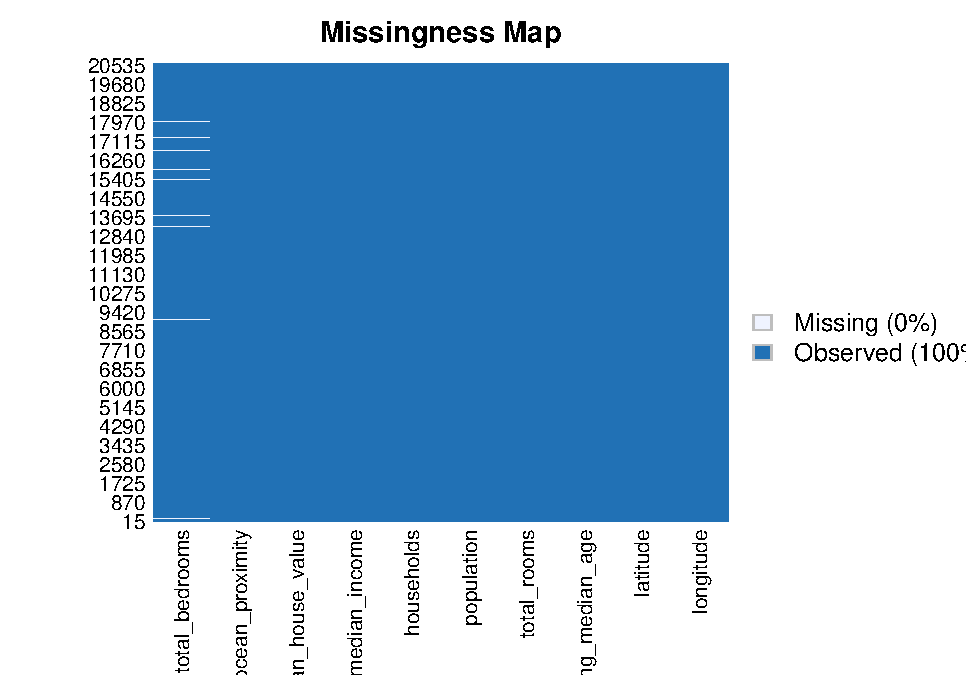
\includegraphics[keepaspectratio]{bookdown-demo_files/figure-latex/datos faltantes opcion2-1.pdf}}

Y ahora se imputan los datos. Hablar de la importancia de imputar los datos blablabla

\begin{Shaded}
\begin{Highlighting}[]
\NormalTok{data }\SpecialCharTok{\%\textgreater{}\%} 
  \FunctionTok{mutate}\NormalTok{(}\FunctionTok{across}\NormalTok{(}
    \FunctionTok{where}\NormalTok{(is.numeric),}
    \SpecialCharTok{\textasciitilde{}} \FunctionTok{ifelse}\NormalTok{(}\FunctionTok{is.na}\NormalTok{(.),}\FunctionTok{mean}\NormalTok{(.,}\AttributeTok{na.rm=}\ConstantTok{TRUE}\NormalTok{),.)}
\NormalTok{  )) }\OtherTok{{-}\textgreater{}}\NormalTok{ df}
\end{Highlighting}
\end{Shaded}

Ahora pues se verifica que, en efecto, la imputación de datos se haya efectuado:

\begin{Shaded}
\begin{Highlighting}[]
\NormalTok{df }\SpecialCharTok{\%\textgreater{}\%}
  \FunctionTok{summarise}\NormalTok{(}\FunctionTok{across}\NormalTok{(}\FunctionTok{everything}\NormalTok{(), }\SpecialCharTok{\textasciitilde{}}\FunctionTok{sum}\NormalTok{(}\FunctionTok{is.na}\NormalTok{(.)),}\AttributeTok{.names=}\StringTok{"NA\_\{.col\}"}\NormalTok{))}
\end{Highlighting}
\end{Shaded}

\begin{verbatim}
##   NA_longitude NA_latitude NA_housing_median_age NA_total_rooms
## 1            0           0                     0              0
##   NA_total_bedrooms NA_population NA_households NA_median_income
## 1                 0             0             0                0
##   NA_median_house_value NA_ocean_proximity
## 1                     0                  0
\end{verbatim}

En efecto.

Ahora se va a convertir la variable de aproximación en oceano. Esto para algo dshfhsfsjf

\begin{Shaded}
\begin{Highlighting}[]
\NormalTok{df}\SpecialCharTok{$}\NormalTok{ocean\_proximity }\OtherTok{\textless{}{-}} \FunctionTok{factor}\NormalTok{ (df}\SpecialCharTok{$}\NormalTok{ocean\_proximity)}
\end{Highlighting}
\end{Shaded}

\chapter{Análisis de la variable median\_house\_value}\label{anuxe1lisis-de-la-variable-median_house_value}

\begin{Shaded}
\begin{Highlighting}[]
\NormalTok{df }\SpecialCharTok{\%\textgreater{}\%} 
  \FunctionTok{summarise}\NormalTok{(}\AttributeTok{n=}\FunctionTok{length}\NormalTok{(median\_house\_value),}
                 \AttributeTok{media=}\FunctionTok{mean}\NormalTok{(median\_house\_value),}
                 \AttributeTok{sd=}\FunctionTok{sd}\NormalTok{(median\_house\_value),}
                 \AttributeTok{mediana=}\FunctionTok{median}\NormalTok{(median\_house\_value),}
                 \AttributeTok{RIC=}\FunctionTok{IQR}\NormalTok{(median\_house\_value),}
                 \AttributeTok{Q1=}\FunctionTok{quantile}\NormalTok{(median\_house\_value,}\FloatTok{0.25}\NormalTok{),}
                 \AttributeTok{Q3=}\FunctionTok{quantile}\NormalTok{(median\_house\_value,}\FloatTok{0.75}\NormalTok{),}
                 \AttributeTok{minimo=}\FunctionTok{min}\NormalTok{(median\_house\_value),}
                 \AttributeTok{maximo=}\FunctionTok{max}\NormalTok{(median\_house\_value),}
                 \AttributeTok{asimetria=}\FunctionTok{skewness}\NormalTok{(median\_house\_value),}
                 \AttributeTok{curtosis=}\FunctionTok{kurtosis}\NormalTok{(median\_house\_value))}
\end{Highlighting}
\end{Shaded}

\begin{verbatim}
##       n    media       sd mediana    RIC     Q1     Q3 minimo maximo asimetria
## 1 20640 206855.8 115395.6  179700 145125 119600 264725  14999 500001 0.9776922
##   curtosis
## 1   3.3275
\end{verbatim}

El número total de casas es de 20640 las cuales tienen un promedio de precio por casa de \$ 206855 (con una desviacion estandar de 115395), podemos afirmar que el 50\% de las casas tienen un valor menor o igual a 179700, ademas tiene un rango intercuartilico de 145125, con un 25\% de las casas con un precio menor o igual a 119.600, y un 75\% por debajo o igual a 264725.

\begin{Shaded}
\begin{Highlighting}[]
\NormalTok{df }\SpecialCharTok{\%\textgreater{}\%} 
  \FunctionTok{ggplot}\NormalTok{(}\FunctionTok{aes}\NormalTok{(}\AttributeTok{x=}\NormalTok{median\_house\_value))}\SpecialCharTok{+}
  \FunctionTok{geom\_histogram}\NormalTok{(}\FunctionTok{aes}\NormalTok{(}\AttributeTok{y=}\FunctionTok{after\_stat}\NormalTok{(density)),}
                 \AttributeTok{binwidth=}\DecValTok{25000}\NormalTok{,}
                 \AttributeTok{fill=}\StringTok{"\#54878f"}\NormalTok{,}
                 \AttributeTok{color=}\StringTok{"white"}\NormalTok{,}
                 \AttributeTok{alpha=}\FloatTok{0.6}\NormalTok{)}\SpecialCharTok{+}
  \FunctionTok{geom\_density}\NormalTok{(}\AttributeTok{color=}\StringTok{"darkblue"}\NormalTok{, }\AttributeTok{linewidth=}\FloatTok{1.2}\NormalTok{)}\SpecialCharTok{+}
  \FunctionTok{labs}\NormalTok{(}\AttributeTok{title=}\StringTok{\textquotesingle{}Distribucion del valor medio de las viviendas\textquotesingle{}}\NormalTok{,}
       \AttributeTok{x=}\StringTok{\textquotesingle{}valor medio de la casa(USD)\textquotesingle{}}\NormalTok{,}
       \AttributeTok{y=}\StringTok{\textquotesingle{}densidad\textquotesingle{}}\NormalTok{)}\SpecialCharTok{+}
  \FunctionTok{theme\_minimal}\NormalTok{()}
\end{Highlighting}
\end{Shaded}

\pandocbounded{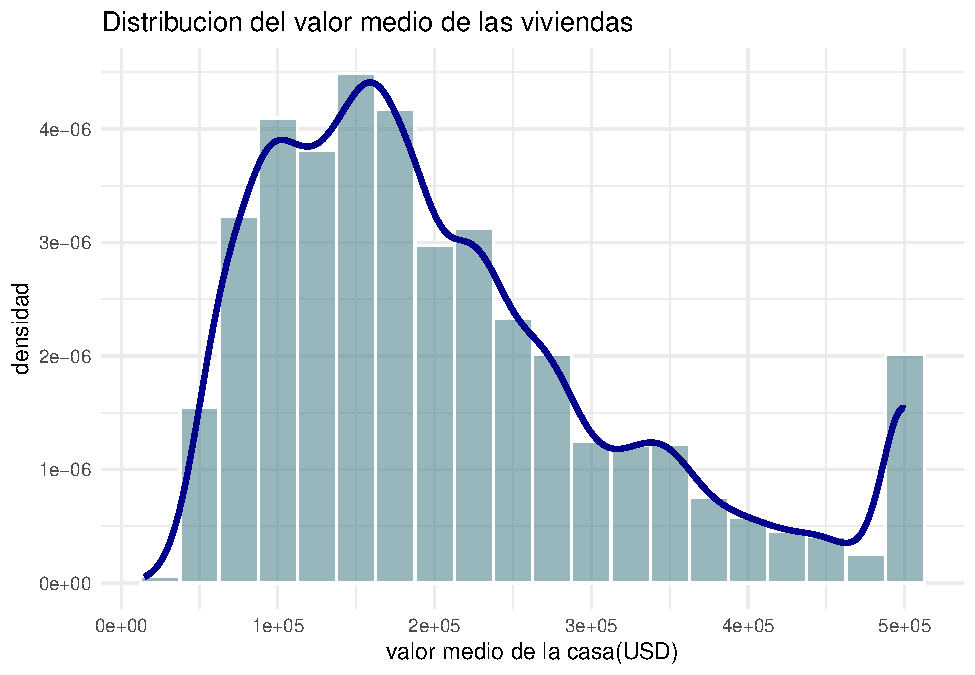
\includegraphics[keepaspectratio]{bookdown-demo_files/figure-latex/histograma de median_house_value-1.pdf}}

\begin{Shaded}
\begin{Highlighting}[]
\NormalTok{df }\SpecialCharTok{\%\textgreater{}\%} 
  \FunctionTok{ggplot}\NormalTok{(}\FunctionTok{aes}\NormalTok{(}\AttributeTok{x=}\StringTok{""}\NormalTok{, }\AttributeTok{y=}\NormalTok{median\_house\_value))}\SpecialCharTok{+}
  \FunctionTok{geom\_boxplot}\NormalTok{(}\AttributeTok{fill=}\StringTok{"\#54878f"}\NormalTok{, }\AttributeTok{color=}\StringTok{"black"}\NormalTok{,}\AttributeTok{outlier.color=}\StringTok{"darkred"}\NormalTok{)}\SpecialCharTok{+}
  \FunctionTok{stat\_summary}\NormalTok{(}\AttributeTok{fun=}\NormalTok{mean, }\AttributeTok{geom=}\StringTok{\textquotesingle{}point\textquotesingle{}}\NormalTok{, }\AttributeTok{shape=}\DecValTok{20}\NormalTok{, }\AttributeTok{size=}\DecValTok{3}\NormalTok{, }\AttributeTok{color=}\StringTok{"darkgreen"}\NormalTok{)}\SpecialCharTok{+}
  \FunctionTok{theme\_minimal}\NormalTok{()}
\end{Highlighting}
\end{Shaded}

\pandocbounded{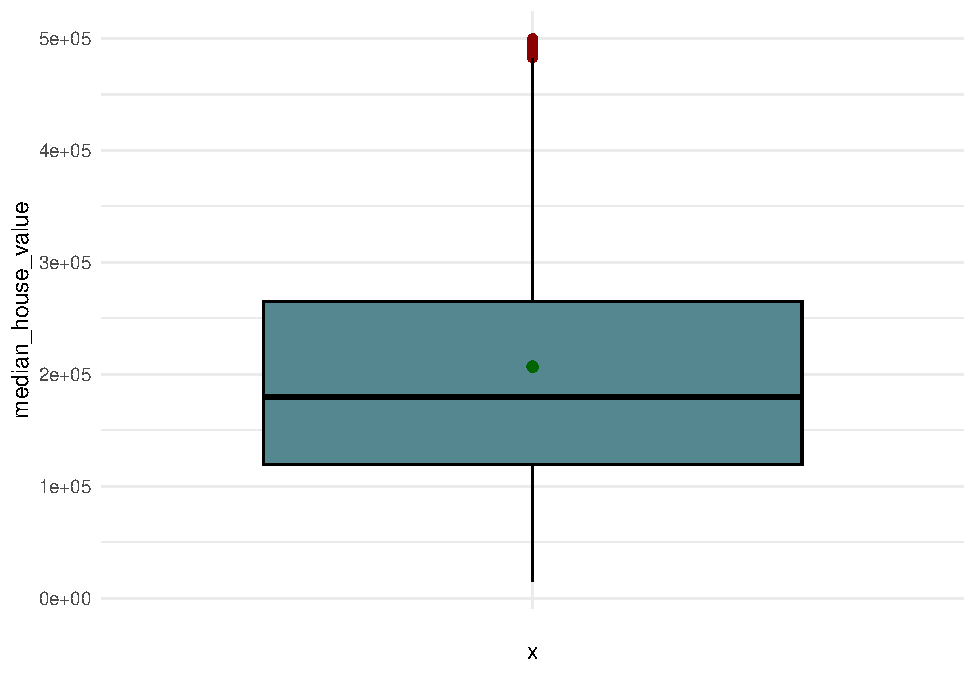
\includegraphics[keepaspectratio]{bookdown-demo_files/figure-latex/histograma de median_house_value-2.pdf}}

El histograma muestra una distribución con asimetría positiva (coeficiente de asimetría de 0.98), es decir, la mayoría de las viviendas se concentran en valores bajos y medios, mientras que unas pocas alcanzan valores muy altos, generando una cola larga hacia la derecha. Se observa además una barra inusualmente alta en \$500.000, correspondiente a 965 viviendas (4.7\% del total), lo que indica que los valores fueron truncados en ese punto.

\begin{Shaded}
\begin{Highlighting}[]
\NormalTok{df }\SpecialCharTok{\%\textgreater{}\%} 
  \FunctionTok{ggplot}\NormalTok{(}\FunctionTok{aes}\NormalTok{(}\AttributeTok{x=}\StringTok{""}\NormalTok{, }\AttributeTok{y=}\NormalTok{median\_house\_value))}\SpecialCharTok{+}
  \FunctionTok{geom\_boxplot}\NormalTok{(}\AttributeTok{fill=}\StringTok{"\#54878f"}\NormalTok{, }\AttributeTok{color=}\StringTok{"black"}\NormalTok{,}\AttributeTok{outlier.color=}\StringTok{"darkred"}\NormalTok{)}\SpecialCharTok{+}
  \FunctionTok{stat\_summary}\NormalTok{(}\AttributeTok{fun=}\NormalTok{mean, }\AttributeTok{geom=}\StringTok{\textquotesingle{}point\textquotesingle{}}\NormalTok{, }\AttributeTok{shape=}\DecValTok{20}\NormalTok{, }\AttributeTok{size=}\DecValTok{3}\NormalTok{, }\AttributeTok{color=}\StringTok{"darkgreen"}\NormalTok{)}\SpecialCharTok{+}
  \FunctionTok{theme\_minimal}\NormalTok{()}
\end{Highlighting}
\end{Shaded}

\pandocbounded{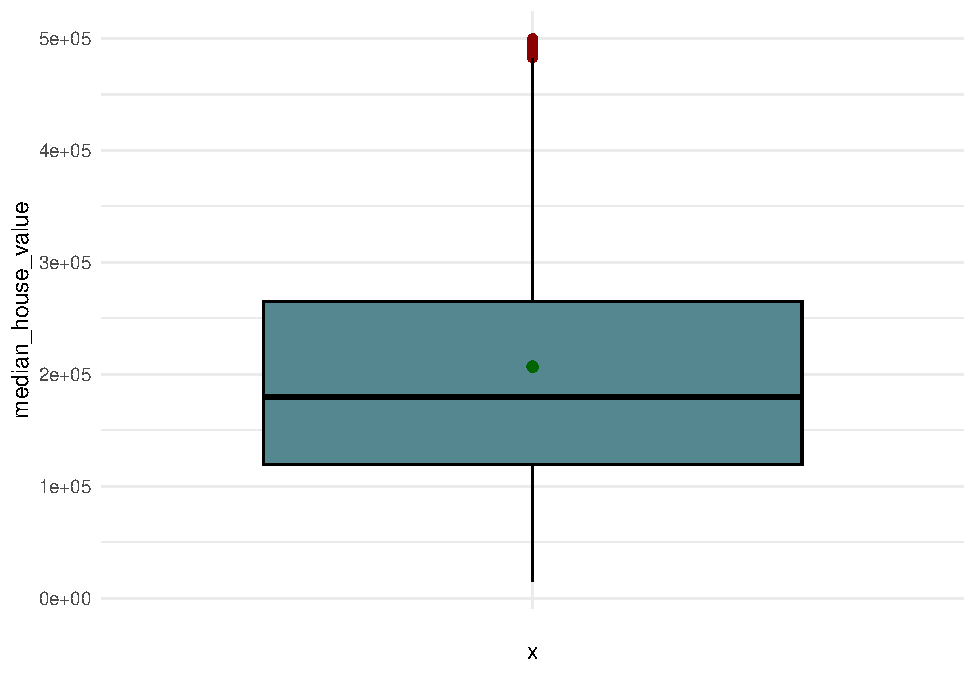
\includegraphics[keepaspectratio]{bookdown-demo_files/figure-latex/caja de bigotes de median_house_value-1.pdf}}

El boxplot confirma la asimetría descrita: la mediana no está centrada dentro de la caja y el bigote superior es más largo que el inferior. Se identifican 1.071 valores atípicos (5.2\% del total), todos por encima del límite superior, lo que refuerza que son las viviendas de mayor valor las que generan la dispersión de la variable.

\chapter{Ánalisis de las variables características (independientes)}\label{uxe1nalisis-de-las-variables-caracteruxedsticas-independientes}

analisis de variables

\begin{Shaded}
\begin{Highlighting}[]
\NormalTok{df }\SpecialCharTok{\%\textgreater{}\%} 
  \FunctionTok{select}\NormalTok{(}\FunctionTok{where}\NormalTok{(is.numeric), }\SpecialCharTok{{-}}\NormalTok{median\_house\_value) }\SpecialCharTok{\%\textgreater{}\%} 
  \FunctionTok{pivot\_longer}\NormalTok{(}
    \AttributeTok{cols=}\FunctionTok{everything}\NormalTok{(),}
    \AttributeTok{names\_to=}\StringTok{\textquotesingle{}variable\textquotesingle{}}\NormalTok{,}
    \AttributeTok{values\_to=}\StringTok{\textquotesingle{}valor\textquotesingle{}}
\NormalTok{  ) }\SpecialCharTok{\%\textgreater{}\%} 
  \FunctionTok{group\_by}\NormalTok{(variable) }\SpecialCharTok{\%\textgreater{}\%}
  \FunctionTok{summarise}\NormalTok{(}\AttributeTok{n=}\FunctionTok{length}\NormalTok{(valor),}
                 \AttributeTok{media=}\FunctionTok{mean}\NormalTok{(valor),}
                 \AttributeTok{sd=}\FunctionTok{sd}\NormalTok{(valor),}
                 \AttributeTok{mediana=}\FunctionTok{median}\NormalTok{(valor),}
                 \AttributeTok{RIC=}\FunctionTok{IQR}\NormalTok{(valor),}
                 \AttributeTok{Q1=}\FunctionTok{quantile}\NormalTok{(valor,}\FloatTok{0.25}\NormalTok{),}
                 \AttributeTok{Q3=}\FunctionTok{quantile}\NormalTok{(valor,}\FloatTok{0.75}\NormalTok{),}
                 \AttributeTok{minimo=}\FunctionTok{min}\NormalTok{(valor),}
                 \AttributeTok{maximo=}\FunctionTok{max}\NormalTok{(valor),}
                 \AttributeTok{asimetria=}\FunctionTok{skewness}\NormalTok{(valor),}
                 \AttributeTok{curtosis=}\FunctionTok{kurtosis}\NormalTok{(valor))}
\end{Highlighting}
\end{Shaded}

\begin{verbatim}
## # A tibble: 8 x 12
##   variable      n   media     sd mediana    RIC      Q1      Q3   minimo  maximo
##   <chr>     <int>   <dbl>  <dbl>   <dbl>  <dbl>   <dbl>   <dbl>    <dbl>   <dbl>
## 1 househol~ 20640  500.   3.82e2  409    3.25e2  280     605       1      6082  
## 2 housing_~ 20640   28.6  1.26e1   29    1.9 e1   18      37       1        52  
## 3 latitude  20640   35.6  2.14e0   34.3  3.78e0   33.9    37.7    32.5      42.0
## 4 longitude 20640 -120.   2.00e0 -118.   3.79e0 -122.   -118.   -124.     -114. 
## 5 median_i~ 20640    3.87 1.90e0    3.53 2.18e0    2.56    4.74    0.500    15.0
## 6 populati~ 20640 1425.   1.13e3 1166    9.38e2  787    1725       3     35682  
## 7 total_be~ 20640  538.   4.19e2  438    3.46e2  297     643.      1      6445  
## 8 total_ro~ 20640 2636.   2.18e3 2127    1.70e3 1448.   3148       2     39320  
## # i 2 more variables: asimetria <dbl>, curtosis <dbl>
\end{verbatim}

INTERPRETACIÓN

\begin{Shaded}
\begin{Highlighting}[]
\NormalTok{df }\SpecialCharTok{\%\textgreater{}\%}
  \FunctionTok{ggplot}\NormalTok{(}\FunctionTok{aes}\NormalTok{(}\AttributeTok{x=}\StringTok{""}\NormalTok{, }\AttributeTok{y=}\NormalTok{housing\_median\_age))}\SpecialCharTok{+}
  \FunctionTok{geom\_boxplot}\NormalTok{(}\AttributeTok{fill=}\StringTok{"\#54878f"}\NormalTok{, }\AttributeTok{color=}\StringTok{"black"}\NormalTok{,}\AttributeTok{outlier.color=}\StringTok{"darkred"}\NormalTok{)}\SpecialCharTok{+}
  \FunctionTok{stat\_summary}\NormalTok{(}\AttributeTok{fun=}\NormalTok{mean, }\AttributeTok{geom=}\StringTok{\textquotesingle{}point\textquotesingle{}}\NormalTok{, }\AttributeTok{shape=}\DecValTok{20}\NormalTok{, }\AttributeTok{size=}\DecValTok{3}\NormalTok{, }\AttributeTok{color=}\StringTok{"darkgreen"}\NormalTok{)}\SpecialCharTok{+}
  \FunctionTok{theme\_minimal}\NormalTok{()}\OtherTok{{-}\textgreater{}}\NormalTok{p1}
\NormalTok{df }\SpecialCharTok{\%\textgreater{}\%}
  \FunctionTok{ggplot}\NormalTok{(}\FunctionTok{aes}\NormalTok{(}\AttributeTok{x=}\StringTok{""}\NormalTok{, }\AttributeTok{y=}\NormalTok{total\_rooms))}\SpecialCharTok{+}
  \FunctionTok{geom\_boxplot}\NormalTok{(}\AttributeTok{fill=}\StringTok{"\#54878f"}\NormalTok{, }\AttributeTok{color=}\StringTok{"black"}\NormalTok{,}\AttributeTok{outlier.color=}\StringTok{"darkred"}\NormalTok{)}\SpecialCharTok{+}
  \FunctionTok{stat\_summary}\NormalTok{(}\AttributeTok{fun=}\NormalTok{mean, }\AttributeTok{geom=}\StringTok{\textquotesingle{}point\textquotesingle{}}\NormalTok{, }\AttributeTok{shape=}\DecValTok{20}\NormalTok{, }\AttributeTok{size=}\DecValTok{3}\NormalTok{, }\AttributeTok{color=}\StringTok{"darkgreen"}\NormalTok{)}\SpecialCharTok{+}
  \FunctionTok{theme\_minimal}\NormalTok{()}\OtherTok{{-}\textgreater{}}\NormalTok{p2}
\NormalTok{df }\SpecialCharTok{\%\textgreater{}\%}
  \FunctionTok{ggplot}\NormalTok{(}\FunctionTok{aes}\NormalTok{(}\AttributeTok{x=}\StringTok{""}\NormalTok{, }\AttributeTok{y=}\NormalTok{total\_bedrooms))}\SpecialCharTok{+}
  \FunctionTok{geom\_boxplot}\NormalTok{(}\AttributeTok{fill=}\StringTok{"\#54878f"}\NormalTok{, }\AttributeTok{color=}\StringTok{"black"}\NormalTok{,}\AttributeTok{outlier.color=}\StringTok{"darkred"}\NormalTok{)}\SpecialCharTok{+}
  \FunctionTok{stat\_summary}\NormalTok{(}\AttributeTok{fun=}\NormalTok{mean, }\AttributeTok{geom=}\StringTok{\textquotesingle{}point\textquotesingle{}}\NormalTok{, }\AttributeTok{shape=}\DecValTok{20}\NormalTok{, }\AttributeTok{size=}\DecValTok{3}\NormalTok{, }\AttributeTok{color=}\StringTok{"darkgreen"}\NormalTok{)}\SpecialCharTok{+}
  \FunctionTok{theme\_minimal}\NormalTok{()}\OtherTok{{-}\textgreater{}}\NormalTok{p3}

\NormalTok{p1}\SpecialCharTok{+}\NormalTok{p2}\SpecialCharTok{+}\NormalTok{p3}
\end{Highlighting}
\end{Shaded}

\pandocbounded{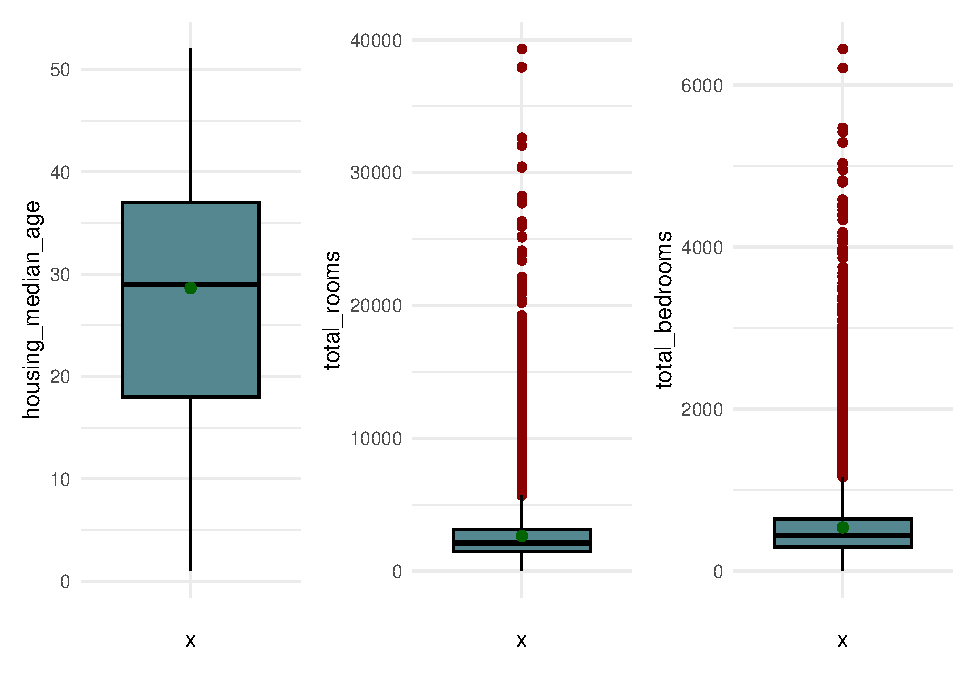
\includegraphics[keepaspectratio]{bookdown-demo_files/figure-latex/análisis variables independientes-1.pdf}}

El número total de observaciones es de 20.640 para cada variable. Para housing\_median\_age, el promedio es de 28.64 años (con una desviación estándar de 12.59), podemos afirmar que el 50\% de las viviendas tienen una antigüedad menor o igual a 29 años, con un rango intercuartílico de 19, un 25\% con antigüedad menor o igual a 18 años y un 75\% por debajo o igual a 37 años.

Para total\_rooms, el promedio es de 2.635.76 habitaciones (con una desviación estándar de 2.181.62), podemos afirmar que el 50\% de los bloques tienen 2.127 habitaciones o menos, con un rango intercuartílico de 1.700.25, un 25\% con 1.447.75 habitaciones o menos y un 75\% por debajo o igual a 3.148.

Para total\_bedrooms, el promedio es de 537.87 dormitorios (con una desviación estándar de 419.27), el 50\% de los bloques tiene 438 dormitorios o menos, con un rango intercuartílico de 346.25, un 25\% con 297 o menos y un 75\% por debajo o igual a 643.25.

Para population, el promedio es de 1.425.48 habitantes (con una desviación estándar de 1.132.46), el 50\% de los bloques tiene 1.166 habitantes o menos, con un rango intercuartílico de 938, un 25\% con 787 o menos y un 75\% por debajo o igual a 1.725.

Para households, el promedio es de 499.54 hogares (con una desviación estándar de 382.33), el 50\% de los bloques tiene 409 hogares o menos, con un rango intercuartílico de 325, un 25\% con 280 o menos y un 75\% por debajo o igual a 605.

Para median\_income, el promedio es de 3.87 (decenas de miles de USD, con una desviación estándar de 1.90), el 50\% de los bloques tiene un ingreso medio menor o igual a 3.53, con un rango intercuartílico de 2.18, un 25\% con 2.56 o menos y un 75\% por debajo o igual a 4.74.

En todas menos housing\_median\_age, los coeficientes de asimetría (entre 1.65 y 4.94) confirman colas derechas marcadas, es decir, la mayoría de los valores son bajos y unos pocos bloques concentran valores extremos.

\begin{Shaded}
\begin{Highlighting}[]
\CommentTok{\# Boxplot de housing\_median\_age}
\NormalTok{p1 }\OtherTok{\textless{}{-}}\NormalTok{ df }\SpecialCharTok{\%\textgreater{}\%}
  \FunctionTok{ggplot}\NormalTok{(}\FunctionTok{aes}\NormalTok{(}\AttributeTok{x =} \StringTok{""}\NormalTok{, }\AttributeTok{y =}\NormalTok{ housing\_median\_age)) }\SpecialCharTok{+}
  \FunctionTok{geom\_boxplot}\NormalTok{(}\AttributeTok{fill =} \StringTok{"\#1f77b4"}\NormalTok{, }\AttributeTok{alpha =} \FloatTok{0.7}\NormalTok{) }\SpecialCharTok{+}
  \FunctionTok{labs}\NormalTok{(}
    \AttributeTok{title =} \StringTok{"Antigüedad media de las viviendas"}\NormalTok{,}
    \AttributeTok{y =} \StringTok{"Años"}\NormalTok{,}
    \AttributeTok{x =} \StringTok{""}
\NormalTok{  ) }\SpecialCharTok{+}
  \FunctionTok{theme\_bw}\NormalTok{()}
\end{Highlighting}
\end{Shaded}

\begin{Shaded}
\begin{Highlighting}[]
\NormalTok{p2 }\OtherTok{\textless{}{-}}\NormalTok{ df }\SpecialCharTok{\%\textgreater{}\%}
  \FunctionTok{ggplot}\NormalTok{(}\FunctionTok{aes}\NormalTok{(}\AttributeTok{x =} \StringTok{""}\NormalTok{, }\AttributeTok{y =}\NormalTok{ total\_rooms)) }\SpecialCharTok{+}
  \FunctionTok{geom\_boxplot}\NormalTok{(}\AttributeTok{fill =} \StringTok{"\#2ca02c"}\NormalTok{, }\AttributeTok{alpha =} \FloatTok{0.7}\NormalTok{) }\SpecialCharTok{+}
  \FunctionTok{labs}\NormalTok{(}
    \AttributeTok{title =} \StringTok{"Número total de habitaciones"}\NormalTok{,}
    \AttributeTok{y =} \StringTok{"Habitaciones"}\NormalTok{,}
    \AttributeTok{x =} \StringTok{""}
\NormalTok{  ) }\SpecialCharTok{+}
  \FunctionTok{theme\_bw}\NormalTok{()}
\end{Highlighting}
\end{Shaded}

\begin{Shaded}
\begin{Highlighting}[]
\NormalTok{p3 }\OtherTok{\textless{}{-}}\NormalTok{ df }\SpecialCharTok{\%\textgreater{}\%}
  \FunctionTok{ggplot}\NormalTok{(}\FunctionTok{aes}\NormalTok{(}\AttributeTok{x =} \StringTok{""}\NormalTok{, }\AttributeTok{y =}\NormalTok{ total\_bedrooms)) }\SpecialCharTok{+}
  \FunctionTok{geom\_boxplot}\NormalTok{(}\AttributeTok{fill =} \StringTok{"\#d62728"}\NormalTok{, }\AttributeTok{alpha =} \FloatTok{0.7}\NormalTok{) }\SpecialCharTok{+}
  \FunctionTok{labs}\NormalTok{(}
    \AttributeTok{title =} \StringTok{"Número total de dormitorios"}\NormalTok{,}
    \AttributeTok{y =} \StringTok{"Dormitorios"}\NormalTok{,}
    \AttributeTok{x =} \StringTok{""}
\NormalTok{  ) }\SpecialCharTok{+}
  \FunctionTok{theme\_bw}\NormalTok{()}
\end{Highlighting}
\end{Shaded}

\begin{Shaded}
\begin{Highlighting}[]
\NormalTok{p4 }\OtherTok{\textless{}{-}}\NormalTok{ df }\SpecialCharTok{\%\textgreater{}\%}
  \FunctionTok{ggplot}\NormalTok{(}\FunctionTok{aes}\NormalTok{(}\AttributeTok{x =} \StringTok{""}\NormalTok{, }\AttributeTok{y =}\NormalTok{ population)) }\SpecialCharTok{+}
  \FunctionTok{geom\_boxplot}\NormalTok{(}\AttributeTok{fill =} \StringTok{"\#9467bd"}\NormalTok{, }\AttributeTok{alpha =} \FloatTok{0.7}\NormalTok{) }\SpecialCharTok{+}
  \FunctionTok{labs}\NormalTok{(}
    \AttributeTok{title =} \StringTok{"Población"}\NormalTok{,}
    \AttributeTok{y =} \StringTok{"Habitantes"}\NormalTok{,}
    \AttributeTok{x =} \StringTok{""}
\NormalTok{  ) }\SpecialCharTok{+}
  \FunctionTok{theme\_bw}\NormalTok{()}
\end{Highlighting}
\end{Shaded}

\begin{Shaded}
\begin{Highlighting}[]
\NormalTok{p5 }\OtherTok{\textless{}{-}}\NormalTok{ df }\SpecialCharTok{\%\textgreater{}\%}
  \FunctionTok{ggplot}\NormalTok{(}\FunctionTok{aes}\NormalTok{(}\AttributeTok{x =} \StringTok{""}\NormalTok{, }\AttributeTok{y =}\NormalTok{ households)) }\SpecialCharTok{+}
  \FunctionTok{geom\_boxplot}\NormalTok{(}\AttributeTok{fill =} \StringTok{"\#ff7f0e"}\NormalTok{, }\AttributeTok{alpha =} \FloatTok{0.7}\NormalTok{) }\SpecialCharTok{+}
  \FunctionTok{labs}\NormalTok{(}
    \AttributeTok{title =} \StringTok{"Número de hogares"}\NormalTok{,}
    \AttributeTok{y =} \StringTok{"Hogares"}\NormalTok{,}
    \AttributeTok{x =} \StringTok{""}
\NormalTok{  ) }\SpecialCharTok{+}
  \FunctionTok{theme\_bw}\NormalTok{()}
\end{Highlighting}
\end{Shaded}

\begin{Shaded}
\begin{Highlighting}[]
\NormalTok{p6 }\OtherTok{\textless{}{-}}\NormalTok{ df }\SpecialCharTok{\%\textgreater{}\%}
  \FunctionTok{ggplot}\NormalTok{(}\FunctionTok{aes}\NormalTok{(}\AttributeTok{x =} \StringTok{""}\NormalTok{, }\AttributeTok{y =}\NormalTok{ median\_income)) }\SpecialCharTok{+}
  \FunctionTok{geom\_boxplot}\NormalTok{(}\AttributeTok{fill =} \StringTok{"\#8c564b"}\NormalTok{, }\AttributeTok{alpha =} \FloatTok{0.7}\NormalTok{) }\SpecialCharTok{+}
  \FunctionTok{labs}\NormalTok{(}
    \AttributeTok{title =} \StringTok{"Ingreso medio"}\NormalTok{,}
    \AttributeTok{y =} \StringTok{"Ingreso (decenas de miles de USD)"}\NormalTok{,}
    \AttributeTok{x =} \StringTok{""}
\NormalTok{  ) }\SpecialCharTok{+}
  \FunctionTok{theme\_bw}\NormalTok{()}

\NormalTok{p7 }\OtherTok{\textless{}{-}}\NormalTok{ df }\SpecialCharTok{\%\textgreater{}\%}
  \FunctionTok{ggplot}\NormalTok{(}\FunctionTok{aes}\NormalTok{(}\AttributeTok{x =} \StringTok{""}\NormalTok{, }\AttributeTok{y =}\NormalTok{ longitude)) }\SpecialCharTok{+}
  \FunctionTok{geom\_boxplot}\NormalTok{(}\AttributeTok{fill =} \StringTok{"\#e377c2"}\NormalTok{, }\AttributeTok{alpha =} \FloatTok{0.7}\NormalTok{) }\SpecialCharTok{+}
  \FunctionTok{labs}\NormalTok{(}\AttributeTok{title =} \StringTok{"Longitud"}\NormalTok{, }\AttributeTok{y =} \StringTok{"Grados"}\NormalTok{, }\AttributeTok{x =} \StringTok{""}\NormalTok{) }\SpecialCharTok{+}
  \FunctionTok{theme\_bw}\NormalTok{()}

\NormalTok{p8 }\OtherTok{\textless{}{-}}\NormalTok{ df }\SpecialCharTok{\%\textgreater{}\%}
  \FunctionTok{ggplot}\NormalTok{(}\FunctionTok{aes}\NormalTok{(}\AttributeTok{x =} \StringTok{""}\NormalTok{, }\AttributeTok{y =}\NormalTok{ latitude)) }\SpecialCharTok{+}
  \FunctionTok{geom\_boxplot}\NormalTok{(}\AttributeTok{fill =} \StringTok{"\#17becf"}\NormalTok{, }\AttributeTok{alpha =} \FloatTok{0.7}\NormalTok{) }\SpecialCharTok{+}
  \FunctionTok{labs}\NormalTok{(}\AttributeTok{title =} \StringTok{"Latitud"}\NormalTok{, }\AttributeTok{y =} \StringTok{"Grados"}\NormalTok{, }\AttributeTok{x =} \StringTok{""}\NormalTok{) }\SpecialCharTok{+}
  \FunctionTok{theme\_bw}\NormalTok{()}
\end{Highlighting}
\end{Shaded}

housing\_median\_age (p1): La antigüedad promedio de las viviendas es de 28.64 años (DS = 12.59 años), con un rango que va desde 1 hasta 52 años. El boxplot no muestra ningún valor atípico según la regla de 1.5×RIC, y la caja está razonablemente centrada entre el primer cuartil (18 años) y el tercer cuartil (37 años), lo que indica una distribución cercana a la simetría. El hecho de que el máximo se detenga exactamente en 52 años sugiere que esta variable pudo haber sido truncada o agrupada en la recolección de los datos, por lo que no debe interpretarse como un límite natural del fenómeno.

total\_rooms (p2): El número promedio de habitaciones por bloque es de 2.635.76 (DS = 2.181.62), una desviación estándar casi tan grande como la media, lo que ya anticipa una fuerte dispersión. El boxplot confirma esto: se identifican 1.287 valores atípicos (6.24\% del total), todos por encima del bigote superior, con un máximo de 39.320 habitaciones frente a una mediana de apenas 2.127. Esto evidencia que la mayoría de los bloques censales son residenciales típicos, pero unos pocos concentran una cantidad de vivienda mucho mayor a la usual (posiblemente zonas de alta densidad o edificios grandes).

total\_bedrooms (p3): Presenta un comportamiento equivalente al de total\_rooms, como es de esperarse dado que ambas variables están naturalmente correlacionadas. El promedio es de 537.87 dormitorios (DS = 419.27), con 1.306 atípicos (6.33\%) por encima del límite superior y un máximo de 6.445 frente a una mediana de 438. La alta dispersión relativa a la media sugiere, nuevamente, heterogeneidad entre bloques predominantemente pequeños y unos pocos con concentraciones habitacionales muy altas.

population (p4): Es la variable con la dispersión más extrema del conjunto: promedio de 1.425.48 habitantes (DS = 1.132.46) y un máximo de 35.682, muy alejado de la mediana de 1.166. El boxplot muestra 1.196 valores atípicos (5.79\%) y una asimetría muy marcada (coeficiente de asimetría de 4.94), lo que indica que, aunque la mayoría de los bloques censales tienen una población moderada, existen algunos con una densidad poblacional extraordinariamente alta que podrían corresponder a zonas urbanas muy densas o incluso a posibles errores de agregación en los datos.

households (p5): El promedio de hogares por bloque es de 499.54 (DS = 382.33), con 1.220 valores atípicos (5.91\%) por encima de un límite superior de aproximadamente 1.093 y un máximo de 6.082. Su comportamiento es consistente con el de population y total\_rooms, lo cual tiene sentido porque las tres variables están relacionadas con el tamaño poblacional del bloque censal.

median\_income (p6): El ingreso medio por bloque es de 3.87 (equivalente a \$38.700 aproximadamente, ya que está escalada en decenas de miles de USD), con una desviación estándar de 1.90. Se detectan 681 valores atípicos (3.3\%), la menor proporción entre las variables con asimetría marcada, y el máximo se ubica en 15.0001 --- un valor sospechosamente redondo que, al igual que ocurrió con median\_house\_value, sugiere que los ingresos también fueron truncados en ese punto para los bloques más adinerados.

longitude (p7): El promedio es de -119.57° (DS = 2.0°), con un rango entre -124.35° y -114.31°, sin valores atípicos. A diferencia de las variables anteriores, longitude no representa una cantidad que pueda interpretarse como ``alta'' o ``baja'' en sentido económico, sino la ubicación geográfica de cada bloque dentro de California; su ligera asimetría negativa (-0.30) simplemente refleja que hay más bloques censales concentrados hacia el oeste (zona costera, valores más negativos) que hacia el este del estado.

latitude (p8): El promedio es de 35.63° (DS = 2.14°), con un rango entre 32.54° y 41.95° y sin atípicos. Su asimetría positiva moderada (0.47) indica una mayor concentración de bloques en las latitudes bajas del estado (sur de California), coherente con la alta densidad poblacional de la zona de Los Ángeles.

Ahora, veamos la variable `ocean\_proximity'

\begin{Shaded}
\begin{Highlighting}[]
\NormalTok{df }\SpecialCharTok{\%\textgreater{}\%} 
  \FunctionTok{count}\NormalTok{(ocean\_proximity,}\AttributeTok{name=}\StringTok{"n"}\NormalTok{) }\SpecialCharTok{\%\textgreater{}\%} 
  \FunctionTok{mutate}\NormalTok{(}\AttributeTok{Porcentaje=}\FunctionTok{round}\NormalTok{((n}\SpecialCharTok{/}\FunctionTok{sum}\NormalTok{(n))}\SpecialCharTok{*}\DecValTok{100}\NormalTok{,}\DecValTok{2}\NormalTok{),}
         \AttributeTok{variable=}\StringTok{\textquotesingle{}ocean\_proximity\textquotesingle{}}\NormalTok{,}
         \AttributeTok{categoria=}\FunctionTok{as.character}\NormalTok{(ocean\_proximity))}\SpecialCharTok{\%\textgreater{}\%} \FunctionTok{select}\NormalTok{(variable,categoria,n,Porcentaje)}\OtherTok{{-}\textgreater{}}\NormalTok{ tabla\_ocean}

\NormalTok{tabla\_ocean}
\end{Highlighting}
\end{Shaded}

\begin{verbatim}
##          variable  categoria    n Porcentaje
## 1 ocean_proximity  <1H OCEAN 9136      44.26
## 2 ocean_proximity     INLAND 6551      31.74
## 3 ocean_proximity     ISLAND    5       0.02
## 4 ocean_proximity   NEAR BAY 2290      11.09
## 5 ocean_proximity NEAR OCEAN 2658      12.88
\end{verbatim}

La categoría \textless1H OCEAN domina con 44.3\% de los bloques, seguida de INLAND con 31.7\%. NEAR OCEAN (12.9\%) y NEAR BAY (11.1\%) tienen participación moderada, mientras que ISLAND es prácticamente residual: solo 5 observaciones (0.02\%). Esta categoría tan pequeña merece atención especial más adelante --- probablemente convenga excluirla o agruparla en el análisis bivariado/modelado, porque con tan pocas observaciones cualquier estadístico calculado para ese grupo (media, sd) será muy inestable.

\begin{Shaded}
\begin{Highlighting}[]
\NormalTok{tabla\_ocean\_b }\OtherTok{\textless{}{-}}\NormalTok{ df }\SpecialCharTok{\%\textgreater{}\%} 
  \FunctionTok{count}\NormalTok{(ocean\_proximity,}\AttributeTok{name=}\StringTok{"n"}\NormalTok{) }\SpecialCharTok{\%\textgreater{}\%} 
  \FunctionTok{mutate}\NormalTok{(}\AttributeTok{Porcentaje=}\FunctionTok{round}\NormalTok{((n}\SpecialCharTok{/}\FunctionTok{sum}\NormalTok{(n))}\SpecialCharTok{*}\DecValTok{100}\NormalTok{,}\DecValTok{1}\NormalTok{),}
         \AttributeTok{Etiqueta=} \FunctionTok{paste0}\NormalTok{(n,}\StringTok{"("}\NormalTok{,Porcentaje,}\StringTok{"\%)"}\NormalTok{))}
\NormalTok{tabla\_ocean\_b }\SpecialCharTok{\%\textgreater{}\%} 
  \FunctionTok{ggplot}\NormalTok{(}\FunctionTok{aes}\NormalTok{(}\AttributeTok{x=}\NormalTok{ocean\_proximity,}\AttributeTok{y=}\NormalTok{n))}\SpecialCharTok{+}
  \FunctionTok{geom\_col}\NormalTok{(}\AttributeTok{fill=}\StringTok{"\#008b8b"}\NormalTok{,}\AttributeTok{width=}\FloatTok{0.6}\NormalTok{)}\SpecialCharTok{+}
  \FunctionTok{geom\_text}\NormalTok{(}\FunctionTok{aes}\NormalTok{(}\AttributeTok{label=}\NormalTok{Etiqueta),}\AttributeTok{vjust=}\SpecialCharTok{{-}}\FloatTok{0.5}\NormalTok{,}\AttributeTok{size=}\FloatTok{4.5}\NormalTok{)}\SpecialCharTok{+}
  \FunctionTok{facet\_wrap}\NormalTok{(}\SpecialCharTok{\textasciitilde{}}\StringTok{\textquotesingle{}Distribución de la variable ocean proximity\textquotesingle{}}\NormalTok{)}\SpecialCharTok{+}
  \FunctionTok{scale\_y\_continuous}\NormalTok{(}\AttributeTok{expand=}\FunctionTok{expansion}\NormalTok{(}\AttributeTok{mult=}\FunctionTok{c}\NormalTok{(}\DecValTok{0}\NormalTok{,}\FloatTok{0.15}\NormalTok{)))}\SpecialCharTok{+}
  \FunctionTok{theme\_minimal}\NormalTok{()}
\end{Highlighting}
\end{Shaded}

\pandocbounded{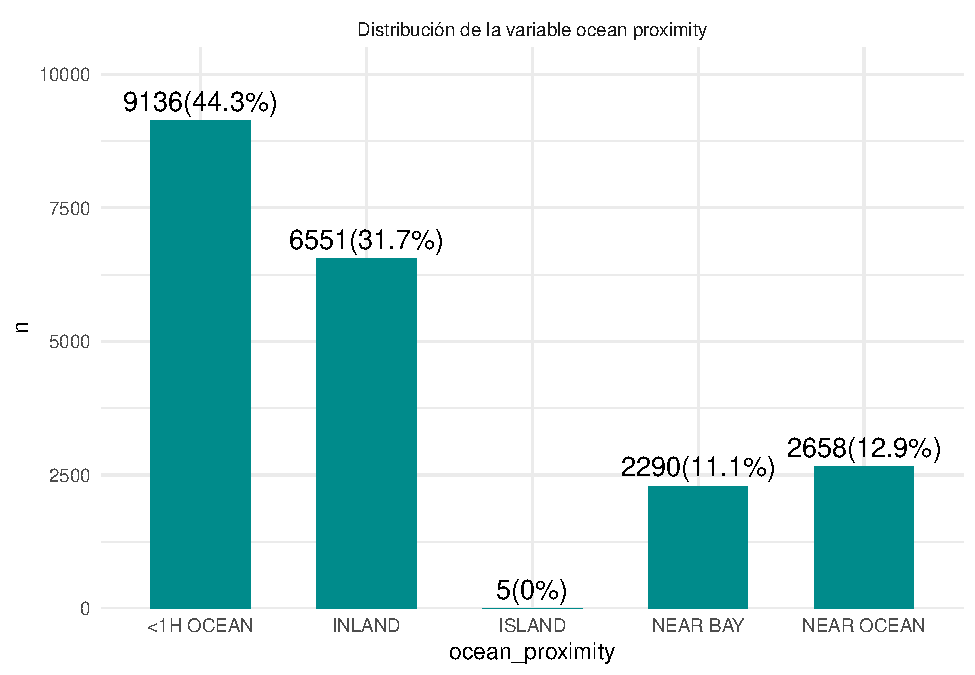
\includegraphics[keepaspectratio]{bookdown-demo_files/figure-latex/unnamed-chunk-5-1.pdf}}

El gráfico confirma visualmente el desbalance: dos categorías (\textless1H OCEAN e INLAND) concentran el 76\% de las observaciones, mientras que ISLAND es casi invisible en la escala del gráfico. Esto sugiere que la variable, aunque útil, tiene una distribución de clases muy desigual --- algo que vale la pena mencionar como limitación del dataset.

\chapter{Ánalisis exploratorio bivariado}\label{uxe1nalisis-exploratorio-bivariado}

\begin{Shaded}
\begin{Highlighting}[]
\NormalTok{df }\SpecialCharTok{\%\textgreater{}\%} 
  \FunctionTok{ggplot}\NormalTok{(}\FunctionTok{aes}\NormalTok{(}\AttributeTok{x=}\NormalTok{median\_income,}\AttributeTok{y=}\NormalTok{median\_house\_value))}\SpecialCharTok{+}
  \FunctionTok{geom\_point}\NormalTok{(}\AttributeTok{alpha=}\FloatTok{0.4}\NormalTok{,}\AttributeTok{color=}\StringTok{\textquotesingle{}darkblue\textquotesingle{}}\NormalTok{)}\SpecialCharTok{+}
  \FunctionTok{labs}\NormalTok{(}\AttributeTok{y=}\StringTok{\textquotesingle{}valor medio de la vivienda\textquotesingle{}}\NormalTok{,}\AttributeTok{x=}\StringTok{\textquotesingle{}ingreso medio\textquotesingle{}}\NormalTok{)}\SpecialCharTok{+}
  \FunctionTok{theme\_minimal}\NormalTok{()}\SpecialCharTok{+}
  \FunctionTok{facet\_grid}\NormalTok{(.}\SpecialCharTok{\textasciitilde{}}\StringTok{\textquotesingle{}Dispersión entre ingreso medio y el valor medio de la vivienda\textquotesingle{}}\NormalTok{)}
\end{Highlighting}
\end{Shaded}

\pandocbounded{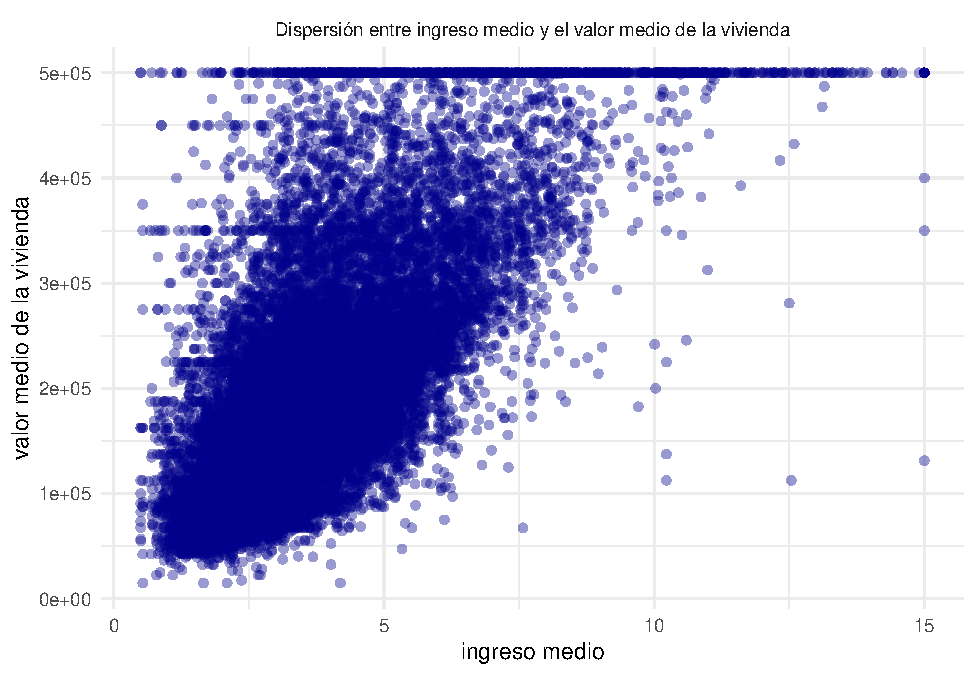
\includegraphics[keepaspectratio]{bookdown-demo_files/figure-latex/valoresingreso-1.pdf}}

\begin{Shaded}
\begin{Highlighting}[]
\NormalTok{df }\SpecialCharTok{\%\textgreater{}\%}
  \FunctionTok{ggplot}\NormalTok{(}\FunctionTok{aes}\NormalTok{(}\AttributeTok{x =}\NormalTok{ housing\_median\_age, }\AttributeTok{y =}\NormalTok{ median\_house\_value)) }\SpecialCharTok{+} \FunctionTok{geom\_point}\NormalTok{(}\AttributeTok{alpha =} \FloatTok{0.4}\NormalTok{, }\AttributeTok{color =} \StringTok{\textquotesingle{}darkblue\textquotesingle{}}\NormalTok{) }\SpecialCharTok{+} \FunctionTok{labs}\NormalTok{(}\AttributeTok{x=}\StringTok{\textquotesingle{}Antigüedad de la vivienda\textquotesingle{}}\NormalTok{, }\AttributeTok{y =} \StringTok{\textquotesingle{}Valor medio de la vivienda\textquotesingle{}}\NormalTok{)}\SpecialCharTok{+} \FunctionTok{theme\_bw}\NormalTok{() }\SpecialCharTok{+} \FunctionTok{facet\_grid}\NormalTok{(.}\SpecialCharTok{\textasciitilde{}} \StringTok{\textquotesingle{}Dispersión entre antigüedad y el valor medio de la vivienda\textquotesingle{}}\NormalTok{)}
\end{Highlighting}
\end{Shaded}

\pandocbounded{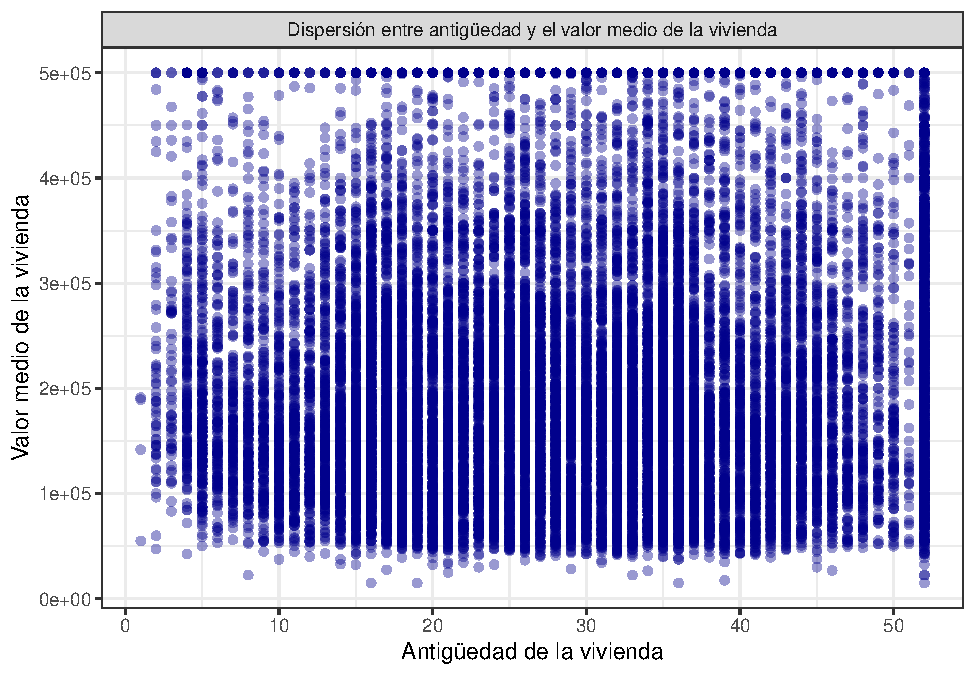
\includegraphics[keepaspectratio]{bookdown-demo_files/figure-latex/housing_median_age vs median_house_value-1.pdf}}

housing\_median\_age vs median\_house\_value: La nube de puntos se distribuye de manera prácticamente uniforme a lo largo de todas las edades, sin que se aprecie una tendencia lineal clara, ni creciente ni decreciente. Para cada valor de antigüedad hay viviendas tanto baratas como caras, lo que sugiere una asociación muy débil entre estas dos variables. Se observa además una línea horizontal de puntos en \$500.000, reflejo del truncamiento ya identificado en el análisis univariado de la variable objetivo.

\begin{Shaded}
\begin{Highlighting}[]
\NormalTok{df }\SpecialCharTok{\%\textgreater{}\%}
  \FunctionTok{ggplot}\NormalTok{(}\FunctionTok{aes}\NormalTok{(}\AttributeTok{x =}\NormalTok{ total\_rooms, }\AttributeTok{y =}\NormalTok{ median\_house\_value)) }\SpecialCharTok{+} \FunctionTok{geom\_point}\NormalTok{(}\AttributeTok{alpha =} \FloatTok{0.4}\NormalTok{, }\AttributeTok{color =} \StringTok{\textquotesingle{}darkblue\textquotesingle{}}\NormalTok{) }\SpecialCharTok{+} \FunctionTok{labs}\NormalTok{(}\AttributeTok{x=}\StringTok{\textquotesingle{}Número total de habitaciones\textquotesingle{}}\NormalTok{, }\AttributeTok{y =} \StringTok{\textquotesingle{}Valor medio de la vivienda\textquotesingle{}}\NormalTok{)}\SpecialCharTok{+} \FunctionTok{theme\_bw}\NormalTok{() }\SpecialCharTok{+} \FunctionTok{facet\_grid}\NormalTok{(.}\SpecialCharTok{\textasciitilde{}} \StringTok{\textquotesingle{}Dispersión entre total de habitaciones y el valor medio de la vivienda\textquotesingle{}}\NormalTok{)}
\end{Highlighting}
\end{Shaded}

\pandocbounded{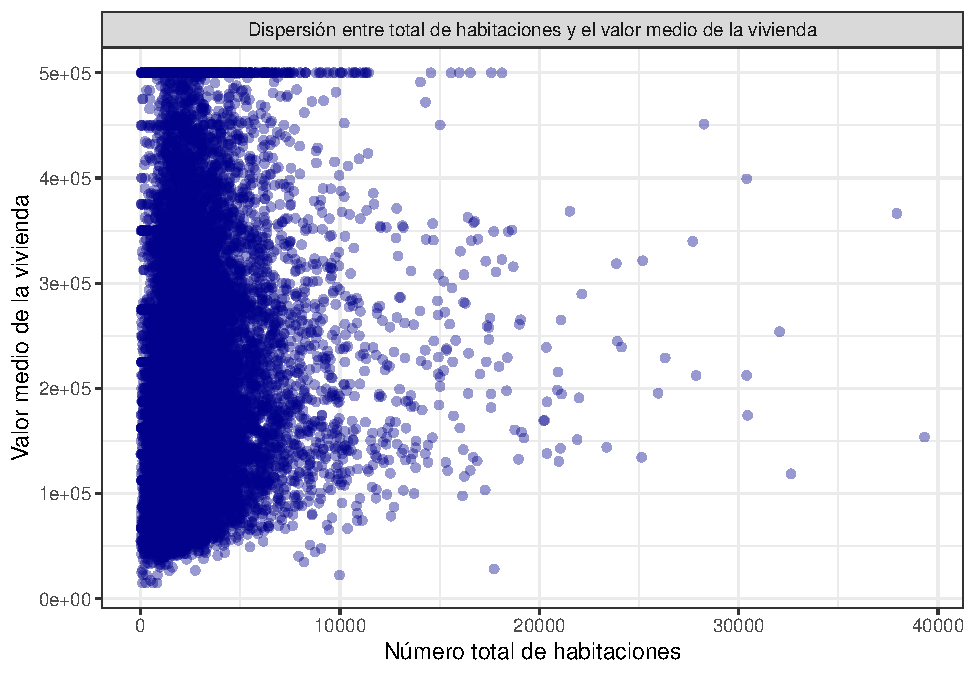
\includegraphics[keepaspectratio]{bookdown-demo_files/figure-latex/total_rooms vs median_house_value-1.pdf}}

total\_rooms vs median\_house\_value: La mayoría de los puntos se concentran en la zona baja del eje X (pocas habitaciones), con una leve tendencia a que el valor de la vivienda aumente conforme crece el número de habitaciones, aunque de forma muy dispersa y con mucho ruido. Se distinguen varios puntos atípicos alejados hacia la derecha (bloques con muchas habitaciones) que no necesariamente corresponden a los valores de vivienda más altos, lo que indica una asociación débil y no estrictamente lineal.

\begin{Shaded}
\begin{Highlighting}[]
\NormalTok{df }\SpecialCharTok{\%\textgreater{}\%}
  \FunctionTok{ggplot}\NormalTok{(}\FunctionTok{aes}\NormalTok{(}\AttributeTok{x =}\NormalTok{ total\_bedrooms, }\AttributeTok{y =}\NormalTok{ median\_house\_value)) }\SpecialCharTok{+} \FunctionTok{geom\_point}\NormalTok{(}\AttributeTok{alpha =} \FloatTok{0.4}\NormalTok{, }\AttributeTok{color =} \StringTok{\textquotesingle{}darkblue\textquotesingle{}}\NormalTok{) }\SpecialCharTok{+} \FunctionTok{labs}\NormalTok{(}\AttributeTok{x=}\StringTok{\textquotesingle{}Número total de dormitorios\textquotesingle{}}\NormalTok{, }\AttributeTok{y =} \StringTok{\textquotesingle{}Valor medio de la vivienda\textquotesingle{}}\NormalTok{)}\SpecialCharTok{+} \FunctionTok{theme\_bw}\NormalTok{() }\SpecialCharTok{+} \FunctionTok{facet\_grid}\NormalTok{(.}\SpecialCharTok{\textasciitilde{}} \StringTok{\textquotesingle{}Dispersión entre total de dormitorios y el valor medio de la vivienda\textquotesingle{}}\NormalTok{)}
\end{Highlighting}
\end{Shaded}

\pandocbounded{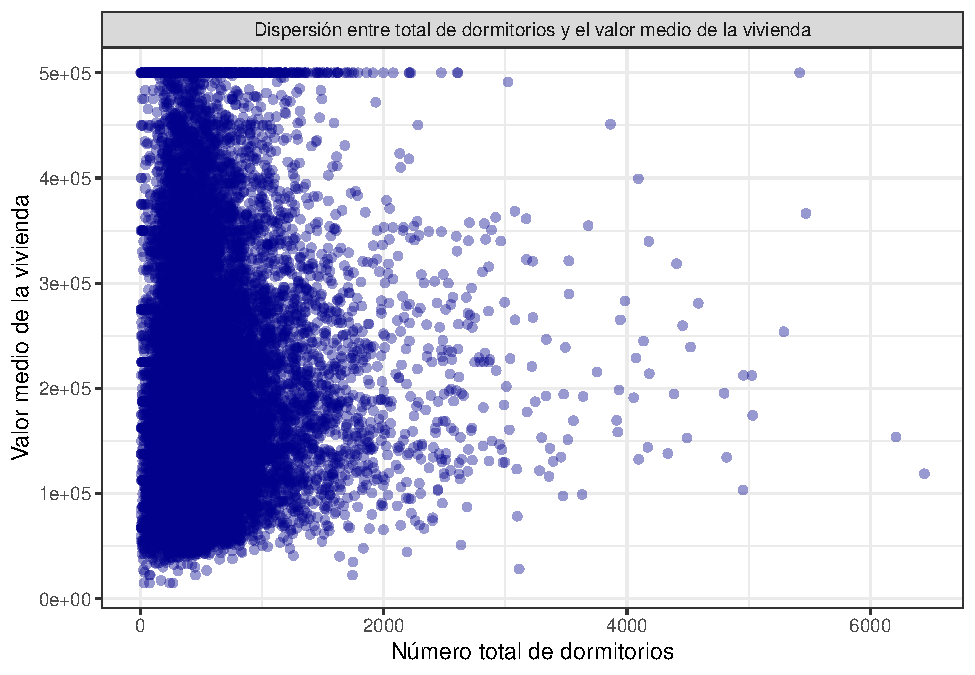
\includegraphics[keepaspectratio]{bookdown-demo_files/figure-latex/total_bedrooms vs median_house_value-1.pdf}}

total\_bedrooms vs median\_house\_value: El patrón es muy similar al anterior: una nube densa y dispersa sin una tendencia definida, con algunos puntos atípicos hacia la derecha (bloques con muchos dormitorios) dispersos en distintos niveles de precio. La asociación visual con la variable objetivo es prácticamente nula.

\begin{Shaded}
\begin{Highlighting}[]
\NormalTok{df }\SpecialCharTok{\%\textgreater{}\%}
  \FunctionTok{ggplot}\NormalTok{(}\FunctionTok{aes}\NormalTok{(}\AttributeTok{x =}\NormalTok{ population, }\AttributeTok{y =}\NormalTok{ median\_house\_value)) }\SpecialCharTok{+} \FunctionTok{geom\_point}\NormalTok{(}\AttributeTok{alpha =} \FloatTok{0.4}\NormalTok{, }\AttributeTok{color =} \StringTok{\textquotesingle{}darkblue\textquotesingle{}}\NormalTok{) }\SpecialCharTok{+} \FunctionTok{labs}\NormalTok{(}\AttributeTok{x=}\StringTok{\textquotesingle{}Población\textquotesingle{}}\NormalTok{, }\AttributeTok{y =} \StringTok{\textquotesingle{}Valor medio de la vivienda\textquotesingle{}}\NormalTok{)}\SpecialCharTok{+} \FunctionTok{theme\_bw}\NormalTok{() }\SpecialCharTok{+} \FunctionTok{facet\_grid}\NormalTok{(.}\SpecialCharTok{\textasciitilde{}} \StringTok{\textquotesingle{}Dispersión entre población y el valor medio de la vivienda\textquotesingle{}}\NormalTok{)}
\end{Highlighting}
\end{Shaded}

\pandocbounded{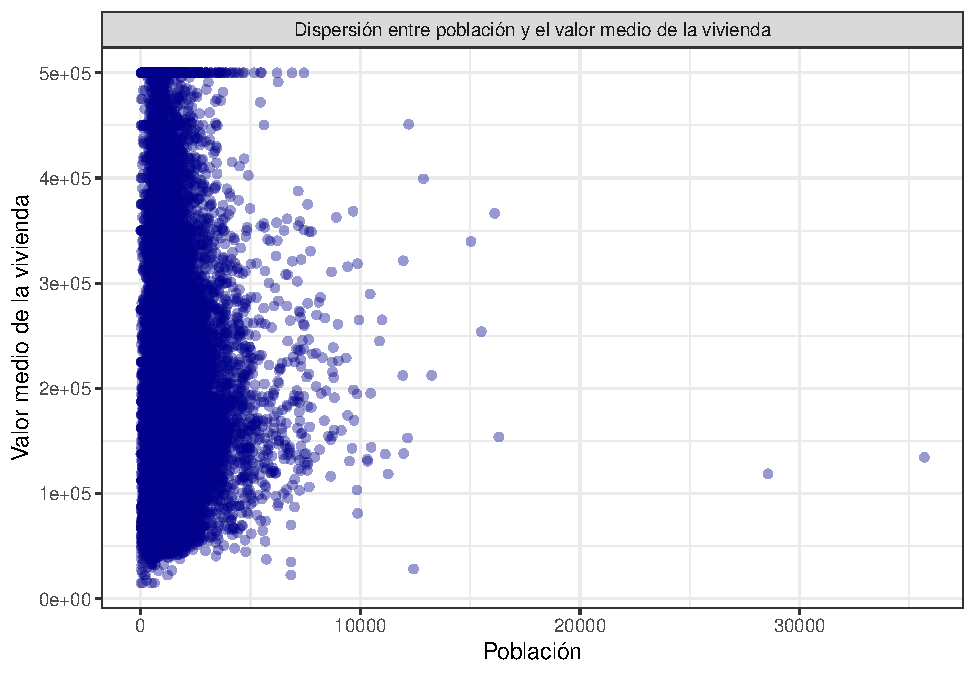
\includegraphics[keepaspectratio]{bookdown-demo_files/figure-latex/population vs median_house_value-1.pdf}}

population vs median\_house\_value: Se observa una nube de puntos muy concentrada en valores bajos de población, con una cola de atípicos que se extiende hacia la derecha (bloques con población extremadamente alta) que no muestran precios particularmente más altos ni más bajos. No hay evidencia visual de una relación lineal entre estas dos variables.

\begin{Shaded}
\begin{Highlighting}[]
\NormalTok{df }\SpecialCharTok{\%\textgreater{}\%}
  \FunctionTok{ggplot}\NormalTok{(}\FunctionTok{aes}\NormalTok{(}\AttributeTok{x =}\NormalTok{ households, }\AttributeTok{y =}\NormalTok{ median\_house\_value)) }\SpecialCharTok{+} \FunctionTok{geom\_point}\NormalTok{(}\AttributeTok{alpha =} \FloatTok{0.4}\NormalTok{, }\AttributeTok{color =} \StringTok{\textquotesingle{}darkblue\textquotesingle{}}\NormalTok{) }\SpecialCharTok{+} \FunctionTok{labs}\NormalTok{(}\AttributeTok{x=}\StringTok{\textquotesingle{}Número de hogares\textquotesingle{}}\NormalTok{, }\AttributeTok{y =} \StringTok{\textquotesingle{}Valor medio de la vivienda\textquotesingle{}}\NormalTok{)}\SpecialCharTok{+} \FunctionTok{theme\_bw}\NormalTok{() }\SpecialCharTok{+} \FunctionTok{facet\_grid}\NormalTok{(.}\SpecialCharTok{\textasciitilde{}} \StringTok{\textquotesingle{}Dispersión entre número de hogares y el valor medio de la vivienda\textquotesingle{}}\NormalTok{)}
\end{Highlighting}
\end{Shaded}

\pandocbounded{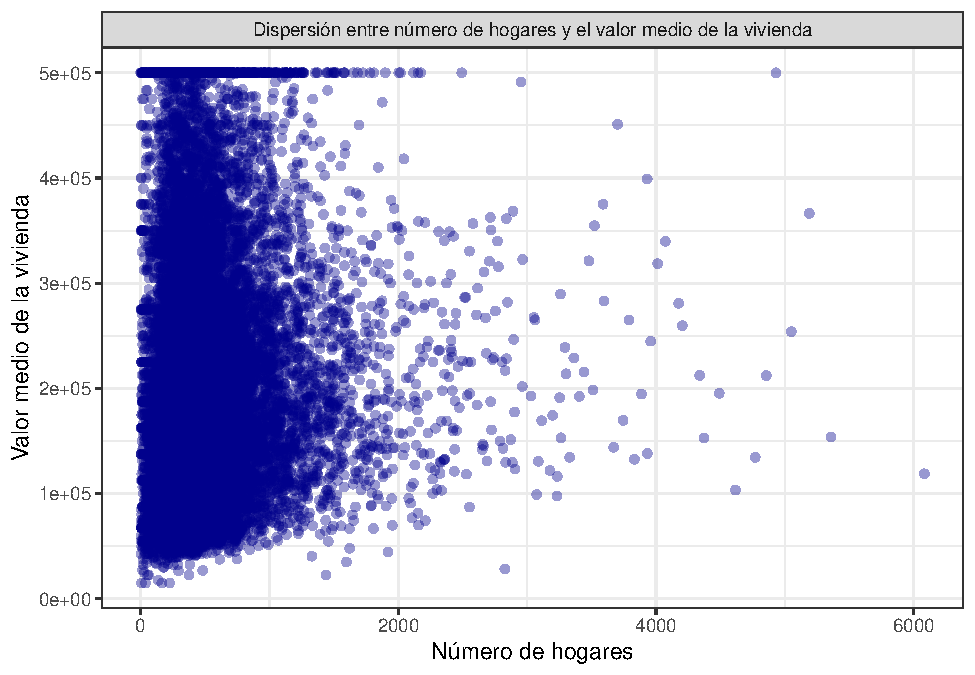
\includegraphics[keepaspectratio]{bookdown-demo_files/figure-latex/households vs median_house_value-1.pdf}}

households vs median\_house\_value: Al igual que con population y total\_rooms, la mayoría de los puntos se agrupan en la parte baja del eje X, con atípicos dispersos hacia la derecha. No se aprecia una tendencia lineal clara ni una asociación fuerte con el valor de la vivienda.

\begin{Shaded}
\begin{Highlighting}[]
\NormalTok{df }\SpecialCharTok{\%\textgreater{}\%}
  \FunctionTok{ggplot}\NormalTok{(}\FunctionTok{aes}\NormalTok{(}\AttributeTok{x =}\NormalTok{ longitude, }\AttributeTok{y =}\NormalTok{ median\_house\_value)) }\SpecialCharTok{+} \FunctionTok{geom\_point}\NormalTok{(}\AttributeTok{alpha =} \FloatTok{0.4}\NormalTok{, }\AttributeTok{color =} \StringTok{\textquotesingle{}darkblue\textquotesingle{}}\NormalTok{) }\SpecialCharTok{+} \FunctionTok{labs}\NormalTok{(}\AttributeTok{x=}\StringTok{\textquotesingle{}Longitud\textquotesingle{}}\NormalTok{, }\AttributeTok{y =} \StringTok{\textquotesingle{}Valor medio de la vivienda\textquotesingle{}}\NormalTok{)}\SpecialCharTok{+} \FunctionTok{theme\_bw}\NormalTok{() }\SpecialCharTok{+} \FunctionTok{facet\_grid}\NormalTok{(.}\SpecialCharTok{\textasciitilde{}} \StringTok{\textquotesingle{}Dispersión entre longitud y el valor medio de la vivienda\textquotesingle{}}\NormalTok{)}
\end{Highlighting}
\end{Shaded}

\pandocbounded{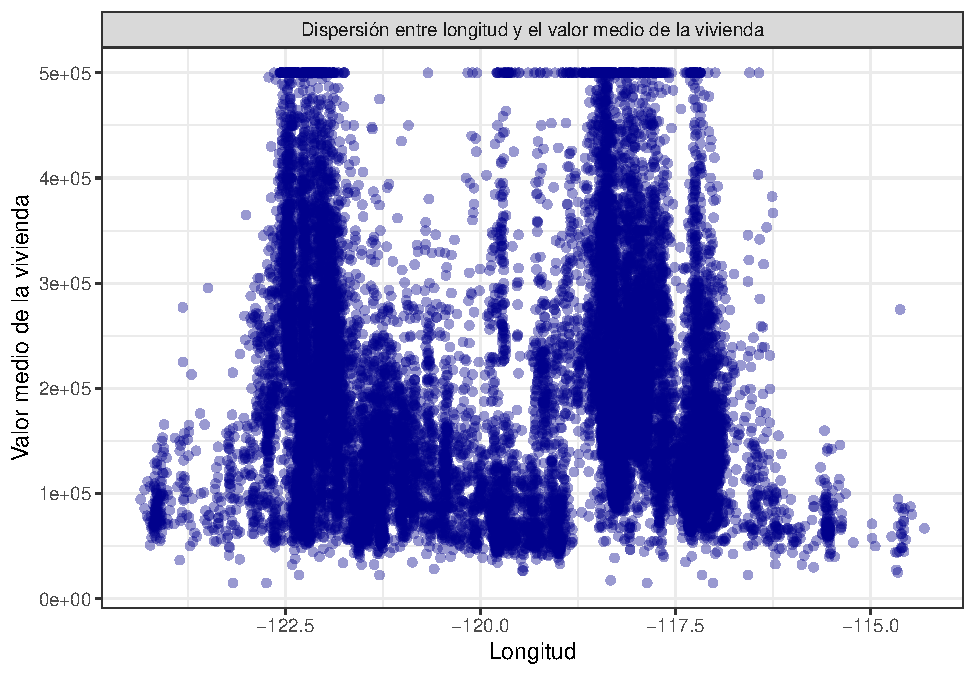
\includegraphics[keepaspectratio]{bookdown-demo_files/figure-latex/longitude vs median_house_value-1.pdf}}

longitude vs median\_house\_value: Aquí el patrón es distinto a los anteriores: en lugar de una tendencia lineal, se observan agrupaciones o ``nubes'' de puntos en ciertos rangos de longitud, con valores de vivienda notablemente más altos alrededor de -122° y -118° (coincidiendo con las zonas de la Bahía de San Francisco y Los Ángeles). Esto sugiere que la relación con median\_house\_value no es lineal, sino que refleja la ubicación geográfica de zonas costeras específicas de mayor valor.

\begin{Shaded}
\begin{Highlighting}[]
\NormalTok{df }\SpecialCharTok{\%\textgreater{}\%}
  \FunctionTok{ggplot}\NormalTok{(}\FunctionTok{aes}\NormalTok{(}\AttributeTok{x =}\NormalTok{ latitude, }\AttributeTok{y =}\NormalTok{ median\_house\_value)) }\SpecialCharTok{+} \FunctionTok{geom\_point}\NormalTok{(}\AttributeTok{alpha =} \FloatTok{0.4}\NormalTok{, }\AttributeTok{color =} \StringTok{\textquotesingle{}darkblue\textquotesingle{}}\NormalTok{) }\SpecialCharTok{+} \FunctionTok{labs}\NormalTok{(}\AttributeTok{x=}\StringTok{\textquotesingle{}Latitud\textquotesingle{}}\NormalTok{, }\AttributeTok{y =} \StringTok{\textquotesingle{}Valor medio de la vivienda\textquotesingle{}}\NormalTok{)}\SpecialCharTok{+} \FunctionTok{theme\_bw}\NormalTok{() }\SpecialCharTok{+} \FunctionTok{facet\_grid}\NormalTok{(.}\SpecialCharTok{\textasciitilde{}} \StringTok{\textquotesingle{}Dispersión entre latitud y el valor medio de la vivienda\textquotesingle{}}\NormalTok{)}
\end{Highlighting}
\end{Shaded}

\pandocbounded{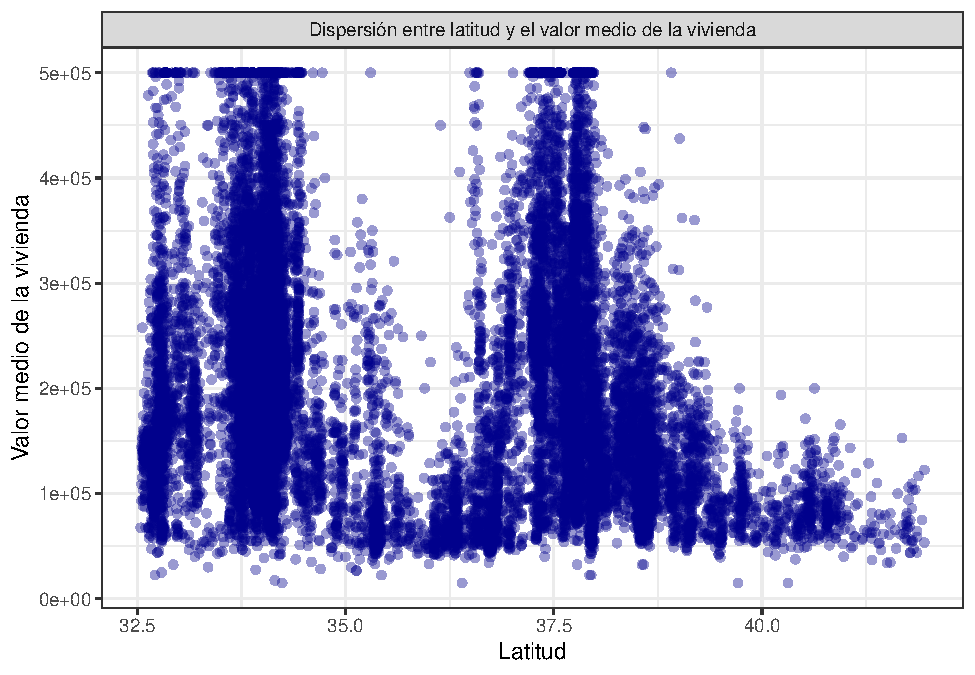
\includegraphics[keepaspectratio]{bookdown-demo_files/figure-latex/latitude vs median_house_value-1.pdf}}

latitude vs median\_house\_value: Se observa un patrón similar al de longitude: no hay una tendencia lineal continua, sino concentraciones de puntos con valores más altos alrededor de las latitudes 34° y 38° (Los Ángeles y la Bahía de San Francisco, respectivamente), y valores más bajos en las latitudes intermedias (zona interior del estado). La relación es de naturaleza geográfica/espacial más que lineal.

Nota general: de las variables analizadas, median\_income es la que muestra la tendencia lineal creciente más clara a simple vista; el resto de variables numéricas (edad, habitaciones, dormitorios, población, hogares) muestran nubes dispersas sin patrón lineal evidente, mientras que longitude y latitude muestran un comportamiento geográfico por zonas en lugar de una tendencia lineal simple.

Ahora comparemos el valor medio de la vivienda según la aproximidad al oceano

\begin{Shaded}
\begin{Highlighting}[]
\NormalTok{df }\SpecialCharTok{\%\textgreater{}\%} 
  \FunctionTok{group\_by}\NormalTok{(ocean\_proximity) }\SpecialCharTok{\%\textgreater{}\%} 
  \FunctionTok{summarise}\NormalTok{(}\AttributeTok{n=}\FunctionTok{length}\NormalTok{(median\_house\_value),}
                 \AttributeTok{media=}\FunctionTok{mean}\NormalTok{(median\_house\_value),}
                 \AttributeTok{sd=}\FunctionTok{sd}\NormalTok{(median\_house\_value),}
                 \AttributeTok{mediana=}\FunctionTok{median}\NormalTok{(median\_house\_value),}
                 \AttributeTok{RIC=}\FunctionTok{IQR}\NormalTok{(median\_house\_value),}
                 \AttributeTok{Q1=}\FunctionTok{quantile}\NormalTok{(median\_house\_value,}\FloatTok{0.25}\NormalTok{),}
                 \AttributeTok{Q3=}\FunctionTok{quantile}\NormalTok{(median\_house\_value,}\FloatTok{0.75}\NormalTok{),}
                 \AttributeTok{minimo=}\FunctionTok{min}\NormalTok{(median\_house\_value),}
                 \AttributeTok{maximo=}\FunctionTok{max}\NormalTok{(median\_house\_value),}
                 \AttributeTok{asimetria=}\FunctionTok{skewness}\NormalTok{(median\_house\_value),}
                 \AttributeTok{curtosis=}\FunctionTok{kurtosis}\NormalTok{(median\_house\_value))}
\end{Highlighting}
\end{Shaded}

\begin{verbatim}
## # A tibble: 5 x 12
##   ocean_proximity     n  media     sd mediana    RIC     Q1     Q3 minimo maximo
##   <fct>           <int>  <dbl>  <dbl>   <dbl>  <dbl>  <dbl>  <dbl>  <dbl>  <dbl>
## 1 <1H OCEAN        9136 2.40e5 1.06e5  214850 125000 164100 289100  17500 500001
## 2 INLAND           6551 1.25e5 7.00e4  108500  71450  77500 148950  14999 500001
## 3 ISLAND              5 3.80e5 8.06e4  414700 150000 300000 450000 287500 450000
## 4 NEAR BAY         2290 2.59e5 1.23e5  233800 183200 162500 345700  22500 500001
## 5 NEAR OCEAN       2658 2.49e5 1.22e5  229450 172750 150000 322750  22500 500001
## # i 2 more variables: asimetria <dbl>, curtosis <dbl>
\end{verbatim}

Falta interpretación

Caja de bigotes

\begin{Shaded}
\begin{Highlighting}[]
\NormalTok{df }\SpecialCharTok{\%\textgreater{}\%} 
\FunctionTok{ggplot}\NormalTok{(}\FunctionTok{aes}\NormalTok{(}\AttributeTok{x=}\NormalTok{ocean\_proximity, }\AttributeTok{y=}\NormalTok{median\_house\_value))}\SpecialCharTok{+}
  \FunctionTok{geom\_boxplot}\NormalTok{(}\AttributeTok{fill=}\StringTok{"\#54878f"}\NormalTok{, }\AttributeTok{color=}\StringTok{"black"}\NormalTok{,}\AttributeTok{outlier.color=}\StringTok{"darkred"}\NormalTok{)}\SpecialCharTok{+}
  \FunctionTok{stat\_summary}\NormalTok{(}\AttributeTok{fun=}\NormalTok{mean, }\AttributeTok{geom=}\StringTok{\textquotesingle{}point\textquotesingle{}}\NormalTok{, }\AttributeTok{shape=}\DecValTok{20}\NormalTok{, }\AttributeTok{size=}\DecValTok{3}\NormalTok{, }\AttributeTok{color=}\StringTok{"darkgreen"}\NormalTok{)}\SpecialCharTok{+}
  \FunctionTok{theme\_minimal}\NormalTok{()}
\end{Highlighting}
\end{Shaded}

\pandocbounded{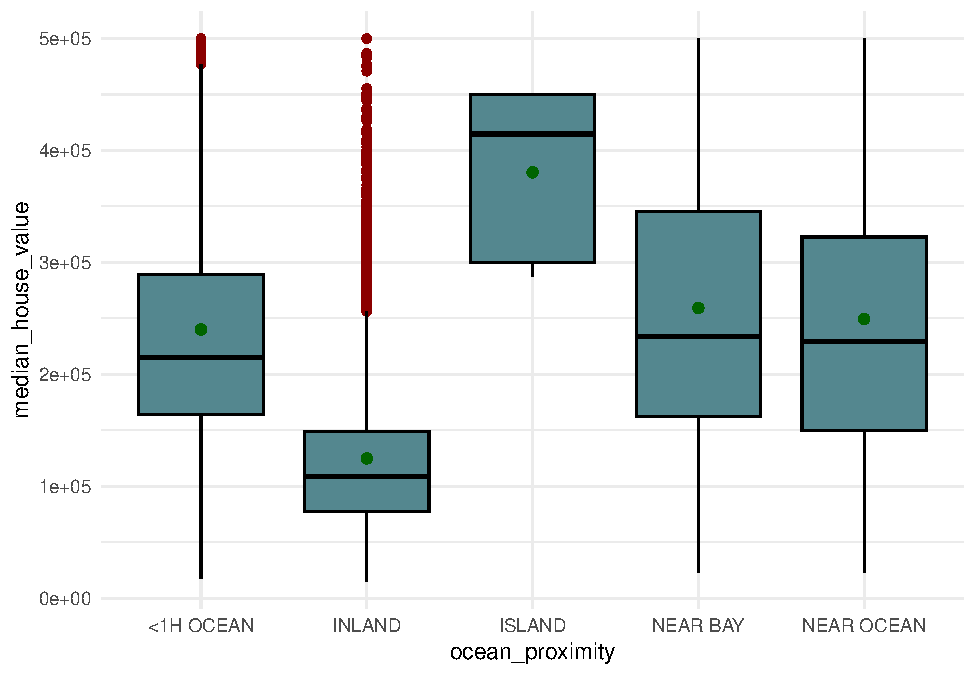
\includegraphics[keepaspectratio]{bookdown-demo_files/figure-latex/unnamed-chunk-6-1.pdf}}
Interpretación

\begin{Shaded}
\begin{Highlighting}[]
\NormalTok{df }\SpecialCharTok{\%\textgreater{}\%} 
  \FunctionTok{ggpairs}\NormalTok{()}
\end{Highlighting}
\end{Shaded}

\begin{verbatim}
## `stat_bin()` using `bins = 30`. Pick better value `binwidth`.
## `stat_bin()` using `bins = 30`. Pick better value `binwidth`.
## `stat_bin()` using `bins = 30`. Pick better value `binwidth`.
## `stat_bin()` using `bins = 30`. Pick better value `binwidth`.
## `stat_bin()` using `bins = 30`. Pick better value `binwidth`.
## `stat_bin()` using `bins = 30`. Pick better value `binwidth`.
## `stat_bin()` using `bins = 30`. Pick better value `binwidth`.
## `stat_bin()` using `bins = 30`. Pick better value `binwidth`.
## `stat_bin()` using `bins = 30`. Pick better value `binwidth`.
\end{verbatim}

\pandocbounded{
\includegraphics[keepaspectratio]{bookdown-demo_files/figure-latex/no se que es eso-1.pdf}}

\chapter{Ánalisis de las variables respuestas (dependientes)}\label{uxe1nalisis-de-las-variables-respuestas-dependientes}

  \bibliography{book.bib,packages.bib}

\end{document}
